% Figure 2: one field's versions in valid time (across) and recorded time (up). Conceptual.
% Build: tectonic fig2-bitemporal.tex
\documentclass[tikz,border=1pt]{standalone}
\usepackage[T1]{fontenc}
\usepackage{DejaVuSans}
\renewcommand{\familydefault}{\sfdefault}
\usetikzlibrary{arrows.meta,calc}

\definecolor{keel}{HTML}{2a78d6}
\definecolor{ink}{HTML}{0b0b0b}
\definecolor{inktwo}{HTML}{52514e}
\definecolor{muted}{HTML}{898781}
\definecolor{rule}{HTML}{c3c2b7}
\definecolor{greylight}{HTML}{dcdad2}
\definecolor{greymid}{HTML}{a3a198}

\begin{document}
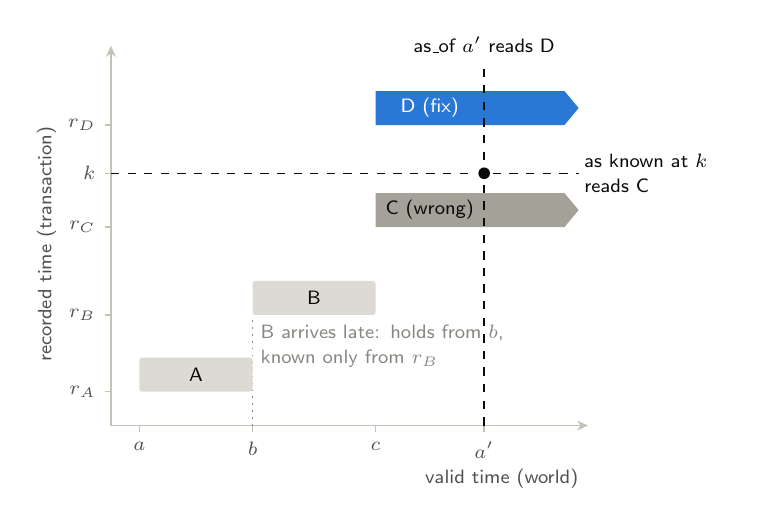
\begin{tikzpicture}[font=\fontsize{7.5}{9}\selectfont, text=inktwo, x=0.6cm, y=0.72cm]
% valid time (x): a, b, c, a'   recorded time (y): rA, rB, rC, k, rD
\def\xa{0.6}\def\xb{3.0}\def\xc{5.6}\def\xq{7.9}\def\xend{9.6}
\def\yA{0.6}\def\yB{1.95}\def\yC{3.5}\def\yk{4.45}\def\yD{5.3}\def\ytop{6.4}
\def\bh{0.6}

% axes
\draw[-{Stealth[length=4pt,width=3.5pt]}, draw=rule, line width=0.6pt] (0,0) -- (\xend+0.5,0);
\draw[-{Stealth[length=4pt,width=3.5pt]}, draw=rule, line width=0.6pt] (0,0) -- (0,\ytop+0.3);
\node[anchor=north east, text=inktwo] at (\xend+0.5,-0.6) {valid time (world)};
\node[anchor=south, rotate=90, text=inktwo] at (-0.95,\ytop/2) {recorded time (transaction)};

% x ticks
\foreach \x/\l in {\xa/{$a$}, \xb/{$b$}, \xc/{$c$}, \xq/{$a'$}} {
  \draw[draw=rule, line width=0.5pt] (\x,0) -- (\x,-0.12);
  \node[anchor=north, text=inktwo] at (\x,-0.12) {\l};
}
% y ticks
\foreach \y/\l in {\yA/{$r_A$}, \yB/{$r_B$}, \yC/{$r_C$}, \yk/{$k$}, \yD/{$r_D$}} {
  \draw[draw=rule, line width=0.5pt] (0,\y) -- (-0.12,\y);
  \node[anchor=east, text=inktwo] at (-0.12,\y) {\l};
}

% B arrived late: it holds from b but was recorded at rB
\draw[draw=muted, dotted, line width=0.5pt] (\xb,0) -- (\xb,\yB);

% versions as horizontal bars: valid interval across, bottom edge at the recorded time
\fill[greylight, rounded corners=1pt] (\xa,\yA) rectangle (\xb,\yA+\bh);
\node[text=ink] at ({(\xa+\xb)/2},\yA+\bh/2) {A};

\fill[greylight, rounded corners=1pt] (\xb,\yB) rectangle (\xc,\yB+\bh);
\node[text=ink] at ({(\xb+\xc)/2},\yB+\bh/2) {B};
\node[anchor=north west, text=muted, text width=3.4cm, align=left, inner sep=1pt]
  at (\xb+0.1,\yB-0.12) {B arrives late: holds from $b$, known only from $r_B$};

% C and D share valid_from = c; both are open-ended (pointed end: no successor yet)
\fill[greymid] (\xc,\yC) -- (\xend,\yC) -- (\xend+0.3,\yC+\bh/2) -- (\xend,\yC+\bh) -- (\xc,\yC+\bh) -- cycle;
\node[text=ink] at ({(\xc+\xq)/2},\yC+\bh/2) {C (wrong)};

\fill[keel] (\xc,\yD) -- (\xend,\yD) -- (\xend+0.3,\yD+\bh/2) -- (\xend,\yD+\bh) -- (\xc,\yD+\bh) -- cycle;
\node[text=white] at ({(\xc+\xq)/2},\yD+\bh/2) {D (fix)};

% as_of a': a vertical read with all knowledge -> D
\draw[draw=ink, dashed, line width=0.5pt] (\xq,0) -- (\xq,\ytop);
\node[anchor=south, text=ink] at (\xq,\ytop) {as\_of $a'$ reads D};

% as known at k: what was believed at recorded time k -> C
\draw[draw=ink, dashed, line width=0.5pt] (0,\yk) -- (\xend+0.3,\yk);
\node[anchor=west, text=ink, text width=2.0cm, align=left, inner sep=1pt] at (\xend+0.35,\yk) {as known at $k$ reads C};
\fill[white] (\xq,\yk) circle (3.2pt);
\fill[ink] (\xq,\yk) circle (2.1pt);

\end{tikzpicture}
\end{document}
